\appendix

\section{Compounding Curve}
\label{sec:compounding_appendix}

\begin{figure}[t]
\centering
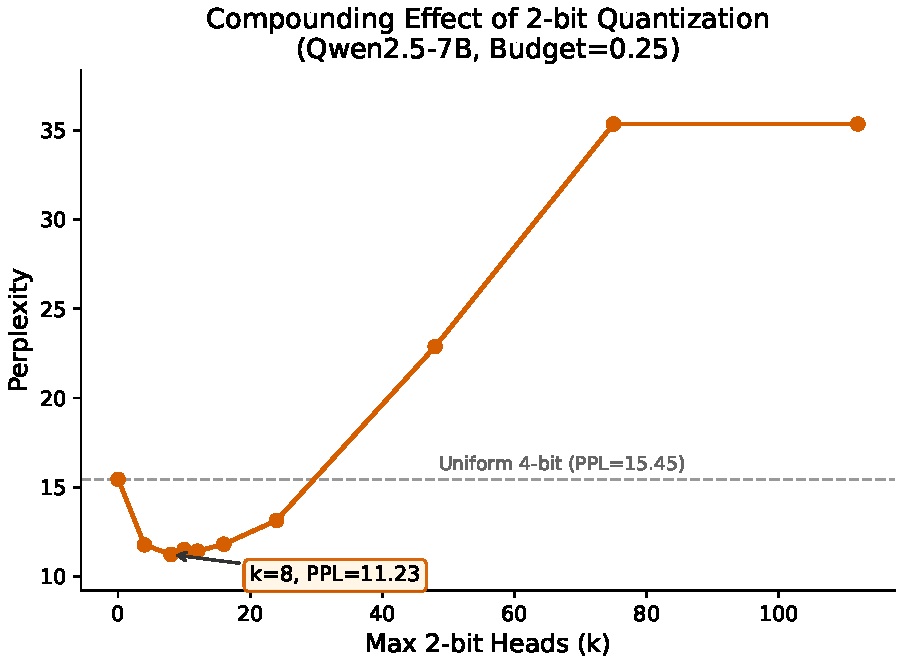
\includegraphics[width=\columnwidth]{figures/fig2_compounding_curve.pdf}
\caption{PPL on Qwen2.5-7B ($4\times$ compression) as a function of $k$, the maximum number of 2-bit heads. Too few 2-bit heads waste budget on 4-bit; too many trigger compounding. The minimum occurs at $k{=}8$.}
\label{fig:compounding}
\end{figure}

\begin{table}[t]
\centering
\small
\caption{Cross-architecture compounding sweep at $4\times$ compression. PPL and degradation relative to the $k{=}0$ baseline ($\times$) as a function of the maximum number of 2-bit heads $k$. Qwen saturates at $k{\approx}96$ due to its 112 KV heads; $k{=}128$ and $k{=}256$ yield identical allocations.}
\label{tab:compounding_sweep}
\begin{tabular}{r cc cc cc}
\toprule
& \multicolumn{2}{c}{Qwen2.5-7B} & \multicolumn{2}{c}{Llama-3.1-8B} & \multicolumn{2}{c}{Mistral-7B-v0.3} \\
\cmidrule(lr){2-3} \cmidrule(lr){4-5} \cmidrule(lr){6-7}
$k$ & PPL & $\times$ & PPL & $\times$ & PPL & $\times$ \\
\midrule
0   & 9.81  & 1.00  & 8.09  & 1.00  & 7.04  & 1.00 \\
2   & 9.83  & 1.00  & 8.12  & 1.00  & 7.04  & 1.00 \\
4   & 9.85  & 1.00  & 8.18  & 1.01  & 7.05  & 1.00 \\
8   & 10.05 & 1.02  & 8.23  & 1.02  & 7.06  & 1.00 \\
16  & 10.40 & 1.06  & 8.44  & 1.04  & 7.11  & 1.01 \\
32  & 11.63 & 1.19  & 9.05  & 1.12  & 7.24  & 1.03 \\
64  & 23.22 & 2.37  & 11.99 & 1.48  & 7.77  & 1.10 \\
128 & 98.75 & 10.1  & 40.21 & 4.97  & 10.47 & 1.49 \\
256 & 98.75 & 10.1  & 1{,}519 & 188  & 45.28 & 6.43 \\
\bottomrule
\end{tabular}
\end{table}

\section{Heuristic Baselines}
\label{sec:heuristic_appendix}

\begin{table}[t]
\centering
\small
\caption{Constrained MCKP vs.\ heuristic baselines at 4$\times$ compression. L0-random reports median and mean$\pm$std over 5 seeds. All methods use per-model optimal $k$ ($k{=}8$ for Qwen, $k{=}2$ for Llama, $k{=}2$ for Mistral). Llama and Mistral use hires profiling. Standard-resolution profiling; hires MCKP achieves 10.91 (Table~\ref{tab:main_results}).}
\label{tab:heuristic}
\begin{tabular}{lcccc}
\toprule
Model & MCKP & \multicolumn{2}{c}{L0-random} & Naive \\
 & & Median & Mean$\pm$Std & Positional \\
\midrule
Qwen2.5-7B      & 11.23 & 11.52 & 11.69$\pm$0.47 & 12.23 \\
Llama-3.1-8B    & 8.45  & 8.62  & 8.62$\pm$0.07  & 8.58 \\
Mistral-7B-v0.3 & 7.13  & 7.20  & 7.24$\pm$0.07  & 7.21 \\
\bottomrule
\end{tabular}
\end{table}

On Qwen, MCKP (11.23) beats the L0-random median (11.52) by 0.29 PPL and the naive positional heuristic (12.23) by 1.00 PPL.
On Llama ($k{=}2$), all methods cluster within 0.17 PPL; on Mistral ($k{=}2$), MCKP (7.13) matches uniform (7.13), while heuristic baselines remain slightly worse.
Heuristic baselines use a slightly higher budget (0.256 vs.\ 0.248, a 3\% difference); despite this advantage, they still underperform MCKP.

\section{Allocation Visualization}
\label{sec:allocation_appendix}

\begin{figure}[t]
\centering
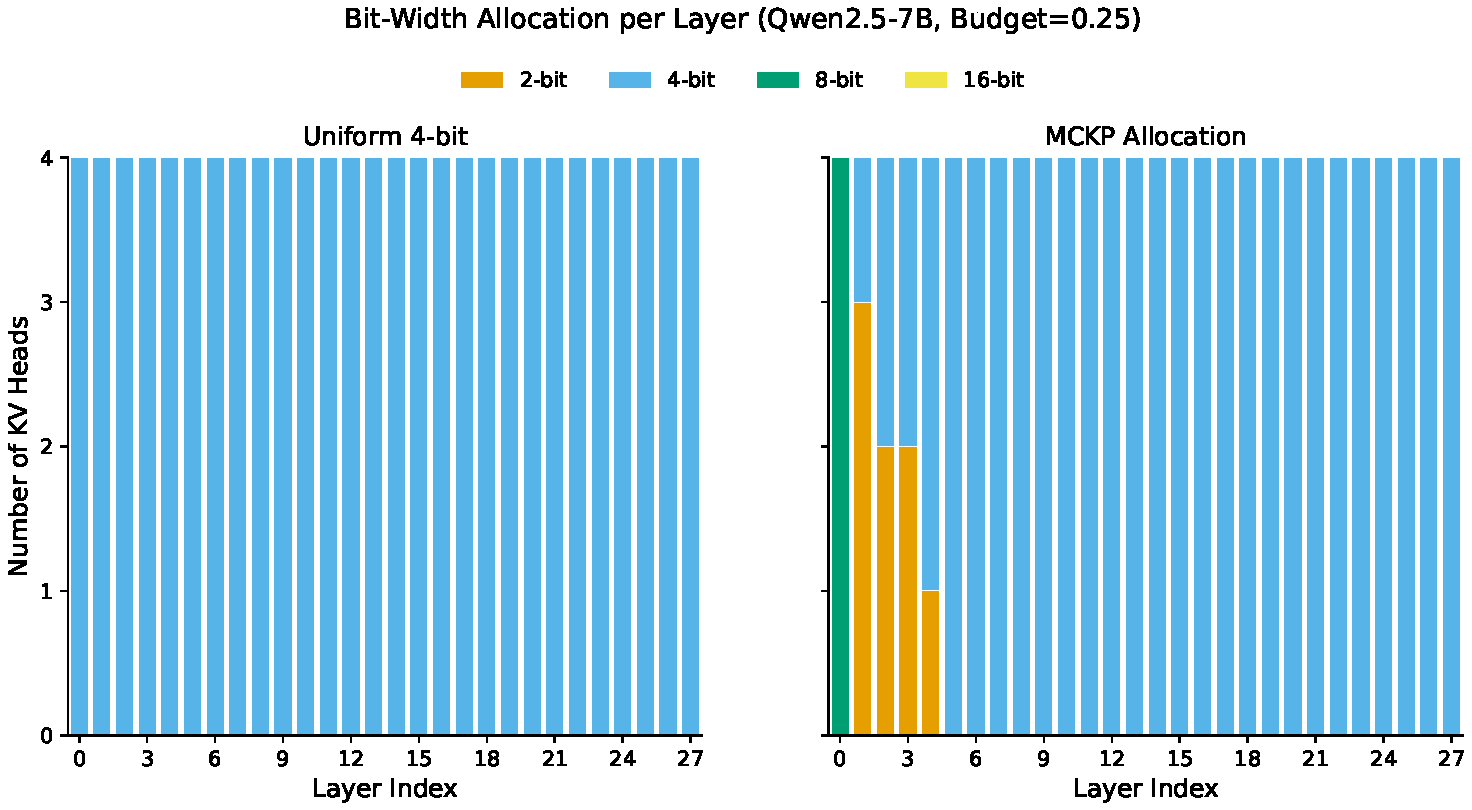
\includegraphics[width=\columnwidth]{figures/fig3_allocation_comparison.pdf}
\caption{Bit-width allocation on Qwen2.5-7B at 4$\times$ compression. Uniform assigns all heads to 4-bit. Constrained MCKP protects Layer-0 heads at 8-bit and assigns the 8 least-sensitive heads to 2-bit.}
\label{fig:allocation}
\end{figure}

\section{Per-Head Sensitivity Heatmap}
\label{sec:heatmap_appendix}

\begin{figure*}[t]
\centering
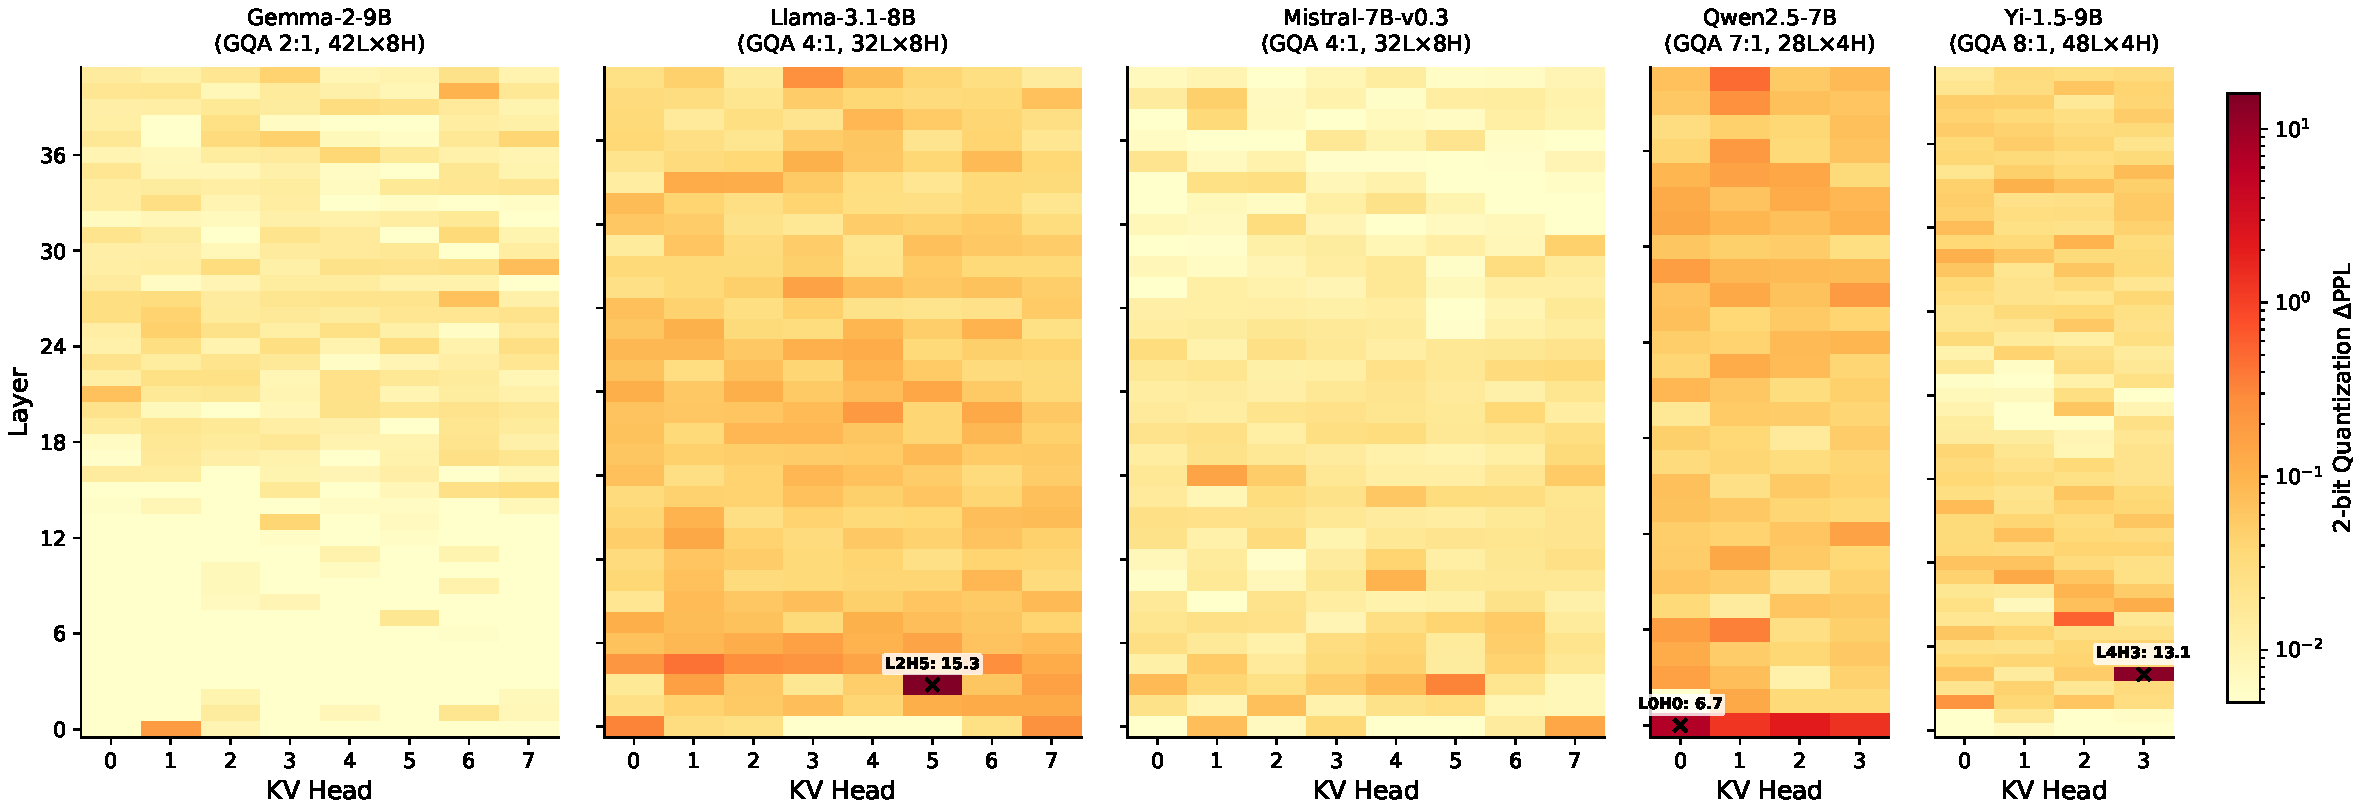
\includegraphics[width=\textwidth]{figures/fig1_head_delta_heatmap.pdf}
\caption{Per-head 2-bit quantization sensitivity across five architectures. Qwen2.5-7B shows high concentration in Layer-0 heads (``spread'' pattern); Yi-1.5-9B shows a single extreme outlier at Layer-4 Head-3 (``spike'' pattern); Llama-3.1-8B shows a dominant outlier at Layer-2 Head-5 (49\% of total distortion, ``spike'' pattern); Mistral-7B-v0.3 shows near-zero sensitivity across all heads; Gemma-2-9B exhibits the most uniform distribution, consistent with its low GQA ratio (2:1). Color intensity indicates PPL increase when the head is quantized to 2-bit.}
\label{fig:heatmap}
\end{figure*}

\section{Granularity Tradeoff}
\label{sec:granularity}

Quantization budget can in principle be allocated at three granularities, each with a distinct cost--benefit profile.
\emph{Layer-level} allocation (KVmix~\cite{li2025kvmix}, KVTuner~\cite{li2025kvtuner}) keeps the search space small ($L$ layers) but forces all heads in a layer to share one bitwidth.
This is fundamentally limited when within-layer variance is large: in Qwen2.5-7B Layer-0, per-head 2-bit deltas are 6.74, 2.12, 1.31, and 1.24---a more than $5\times$ spread that any layer-level assignment must average over.
\emph{Per-head} allocation (ours) exposes this heterogeneity to the solver and yields a 29.4\% PPL improvement on Qwen, at the cost of $H$ profiling passes; the cardinality constraint developed in \S\ref{sec:cardinality} renders the choice of solver irrelevant, amortizing the search overhead.
\emph{Token-level} allocation (ZipCache~\cite{he2024zipcache}, KIVI~\cite{liu2024kivi}) is the finest grain available but introduces runtime overhead from online importance scoring.
Importantly, per-head and per-token granularities are orthogonal: a head's bitwidth (static, determined offline) and a token's importance (dynamic, determined online) compose without conflict, so the two can be combined.
Per-head therefore occupies the sweet spot for static allocation---fine enough to capture the head-level heterogeneity that drives MCKP benefit on spread-pattern models, yet free of any per-step runtime cost.

\section{Budget Sweep}
\label{sec:budget_sweep}

\begin{table}[t]
\centering
\small
\caption{Effect of compression ratio on Qwen2.5-7B. Constrained MCKP provides meaningful gains at moderate-to-aggressive compression ($\geq$4$\times$). Standard-resolution profiling.}
\label{tab:budget_sweep}
\begin{tabular}{cccc}
\toprule
Compression & Uniform PPL & Constr.\ MCKP PPL & $\Delta$ PPL \\
\midrule
2$\times$ & 10.10 & 10.66 & $-$0.56 \\
4$\times$ & 15.45 & 11.23 & $+$4.22 \\
8$\times$ & 14{,}759 & 907 & $+$13{,}852 \\
\bottomrule
\end{tabular}
\end{table}

Table~\ref{tab:budget_sweep} shows how the benefit of constrained allocation varies with compression ratio on Qwen2.5-7B.
At 2$\times$ compression, uniform 8-bit quantization is near-lossless (10.10 PPL vs.\ 9.81 bf16); constrained MCKP is slightly worse (10.66) due to unnecessary 2-bit assignments.
At 4$\times$, constrained MCKP reduces PPL from 15.45 to 11.23, a 27.3\% improvement; hires profiling further reduces this to 10.91 (Appendix~\ref{sec:profiling_resolution}).
At 8$\times$, both methods degrade catastrophically, but constrained MCKP (907) is an order of magnitude better than uniform (14{,}759) because the constraint still protects Layer-0 heads.

\section{Cross-Dataset Stability}
\label{sec:cross_dataset}

\begin{table}[t]
\centering
\small
\caption{Cross-dataset stability at $4\times$ compression. \textit{Top:} Qwen2.5-7B PPL under cross-calibration (C4 bf16 baseline: 15.32). \textit{Bottom:} bit-assignment agreement between WikiText-2 and C4 calibrated profiles.}
\label{tab:cross_dataset}
\begin{tabular}{lcccc}
\toprule
\multicolumn{5}{l}{\textit{Cross-calibration PPL (Qwen2.5-7B)}} \\
\midrule
Calibration & Eval set & MCKP & Uniform & Reduction \\
\midrule
WikiText-2 & WikiText-2 & 11.23 & 15.45 & 27\% \\
C4         & WikiText-2 & 11.29 & 15.45 & 27\% \\
WikiText-2 & C4         & 20.56 & 35.42 & 42\% \\
\midrule
\multicolumn{5}{l}{\textit{Bit-assignment agreement (WT2 vs.\ C4 calibration)}} \\
\midrule
\multicolumn{2}{l}{Model} & Agreement & \multicolumn{2}{c}{Matching / Total} \\
\midrule
\multicolumn{2}{l}{Qwen2.5-7B}      & 96.4\% & \multicolumn{2}{c}{108 / 112} \\
\multicolumn{2}{l}{Llama-3.1-8B}    & 97.7\% & \multicolumn{2}{c}{250 / 256} \\
\multicolumn{2}{l}{Mistral-7B-v0.3} & 96.5\% & \multicolumn{2}{c}{247 / 256} \\
\bottomrule
\end{tabular}
\end{table}

To verify that the profiled allocation is not overfit to the calibration corpus, we profile on C4 and evaluate on WikiText-2, and vice versa, at $4\times$ compression.
On Qwen2.5-7B, C4-calibrated MCKP achieves 11.29 PPL on WikiText-2 (vs.\ 15.45 uniform, a 27\% reduction), only 0.06 PPL above the WikiText-2-calibrated result (11.23).
In the reverse direction, WikiText-2-calibrated MCKP achieves 20.56 PPL on the C4 held-out split (vs.\ 35.42 uniform, a 42\% reduction; C4 bf16 baseline on this split is 15.32).
All three models show ${>}96\%$ bit-assignment agreement across calibration sources: Qwen 96.4\% (108/112 heads), Llama 97.7\% (250/256), and Mistral 96.5\% (247/256).
Qwen's agreement is the most informative, as all 112 heads have variable assignments; on Llama, 253 of 256 heads are forced to 4-bit by the $k{=}2$ constraint, inflating agreement.
The cross-dataset results reinforce the heterogeneity-driven narrative: on Qwen, the MCKP benefit is preserved across calibration sources; on Llama and Mistral, the lack of benefit is equally stable---Llama's C4-calibrated MCKP is 0.18 PPL worse than uniform, and Mistral shows similar degradation ($-$0.03 to $-$0.05 PPL).

\section{Aggressive Compression}
\label{sec:aggressive}

At $4\times$ compression, Llama and Mistral show minimal benefit from non-uniform allocation.
At more aggressive ratios, the picture changes: at $5.3\times$ (average 3 bits), constrained MCKP achieves $45\times$ lower PPL than uniform on Llama (57.60 vs.\ 2643.77) and $44\times$ on Mistral (11.91 vs.\ 519.11), because the constraint protects sensitive heads from 2-bit assignment.
At $8\times$, the budget is too constrained for any allocation to preserve quality (both methods degrade catastrophically).
The intermediate regime ($5.3\times$) provides the largest relative benefit.

\section{Profiling Resolution and Stability}
\label{sec:profiling_resolution}

We compare standard-resolution profiling (16 sequences $\times$ 512 tokens) against high-resolution profiling (64 sequences $\times$ 2048 tokens) on Qwen2.5-7B at $4\times$ compression.

High-resolution profiling improves constrained MCKP from 11.23 to 10.91 PPL ($-$0.32 absolute).
Relative to the bf16 baseline (9.81), this reduces the degradation from 1.42 to 1.10, a 22.5\% reduction.
The improvement comes from finer-grained sensitivity estimates: standard profiling detects non-zero 2-bit distortion in 37 of 112 heads, while high-resolution profiling detects 100 of 112 (2.7$\times$ more).

The additional signal changes 8 of 112 head assignments.
High-resolution profiling protects shallow layers (L1--L3) at higher bit-widths while compressing mid-layers (L5--L11) more aggressively---a redistribution that standard profiling misses because its distortion estimates for these heads fall below the noise floor.

\paragraph{Multi-seed stability.}
The profiled allocation is stable across calibration subsets.
Under hires profiling on Qwen2.5-7B, constrained MCKP yields mean PPL $10.99 \pm 0.06$ across 3 random calibration seeds (individual runs: 11.02, 10.90, 11.05), with std/mean below 0.6\%.
The bit distribution is identical across all seeds ($\{$2-bit: 8, 4-bit: 100, 8-bit: 4$\}$), and 101 of 112 heads (90.2\%) receive the same assignment in all three runs.
This stability confirms that the per-head sensitivity ranking is robust to calibration sampling noise.

\paragraph{Numerical precision.}
Float32 profiling (64 $\times$ 2048 tokens) yields an identical constrained allocation and PPL within seed variance (10.89 vs.\ 10.91, $\Delta = 0.02 < \sigma = 0.06$), confirming that bfloat16 precision is sufficient for the profiling step.

\paragraph{Per-layer optimality.}
To validate the additive distortion assumption underlying the MCKP formulation, we compare constrained MCKP against a per-layer brute-force oracle that exhaustively enumerates all $4^4 = 256$ bit-width combinations within each 4-head group on Qwen2.5-7B (hires profiling).
Of the 8 layers admitting multiple feasible allocations, MCKP matches the oracle exactly in 5; the remaining 3 show gaps of 0.018 (Layer~1), 0.014 (Layer~11), and 0.005 (Layer~4) PPL.
All three gaps involve repositioning a 2-bit assignment among heads with near-identical sensitivity within the same layer bit budget.
The negligible total gap ($<0.04$ PPL) confirms that the per-head additive distortion model closely approximates the true layer-level interaction.

\section{KV Separation Ablation}
\label{sec:kv_separation}

We test whether treating K and V caches as independent items in the MCKP solver---allowing different bit-widths for K and V within the same head---improves over joint allocation where K and V share a bit-width.

Joint allocation achieves 10.91 PPL; separated K/V allocation achieves 11.22 ($+$0.31 worse).
The degradation stems from K-side over-compression: the separated solver doubles the maximum number of 2-bit K items to 16 (vs.\ 8 in the joint formulation), since K and V are counted independently against the cardinality constraint.
Meanwhile, V-side distortion is near-zero for most heads, so the solver assigns all V items to 4-bit, concentrating compression entirely on K.

Of the 112 heads, 21 show K$\neq$V asymmetry in the separated allocation, all with K receiving a lower bit-width than V.
This systematic asymmetry suggests that K caches are inherently more compressible than V caches, consistent with the observation that key vectors primarily encode positional information while value vectors carry content.

Joint allocation is sufficient under the current constraint formulation.
Separated K/V allocation with per-side cardinality constraints---limiting 2-bit assignments independently for K and V---is a direction for future work.

\section{Runtime Benchmark}
\label{sec:runtime}

\begin{table}[ht]
\centering
\caption{PyTorch-level latency on Qwen2.5-7B (single NVIDIA RTX PRO 6000 (96\,GB), prompt\_len=256, gen\_len=128, mean of 10 runs). All conditions store KV in bf16 with simulated per-head quantize/dequantize calls; peak GPU memory is identical across rows.}
\label{tab:runtime}
\begin{tabular}{lccc}
\toprule
Condition & Prefill (ms) & Decode (ms/tok) & Throughput (tok/s) \\
\midrule
Baseline bf16       & 45.86 & 33.78 & 29.6 \\
Uniform 4-bit       & 54.25 & 42.46 & 23.6 \\
Constrained MCKP    & 57.03 & 46.09 & 21.8 \\
\bottomrule
\end{tabular}
\end{table}

Table~\ref{tab:runtime} reports end-to-end latency for three KV cache configurations.
Uniform 4-bit quantization adds 25.7\% decode overhead relative to the bf16 baseline (42.46 vs.\ 33.78~ms/tok), reflecting per-head quantize/dequantize calls at every attention step.
Constrained MCKP adds a further 8.5\% over uniform (46.09 vs.\ 42.46~ms/tok), because mixed-precision allocation dispatches different dequantization kernels for 2-bit, 4-bit, and 8-bit heads within the same layer.
The MCKP solver itself runs in ${\sim}5$~ms and is invoked once at initialization, contributing negligibly to end-to-end latency.
Both quantized conditions achieve the same $4\times$ KV cache compression (5.25~MB vs.\ 21~MB at bf16), so the latency difference between uniform and MCKP reflects only the mixed-precision dispatch overhead, not a memory trade-off.

\paragraph{Caveat.}
These measurements use PyTorch-level per-head \texttt{quantize}/\texttt{dequantize} calls and do \emph{not} represent optimized CUDA kernel performance.
Production inference engines such as vLLM and TensorRT-LLM employ fused attention kernels that batch dequantization with the matrix multiply, amortizing the per-head dispatch cost that dominates the gap between uniform and MCKP in our simulation.
The 8.5\% overhead reported here should therefore be treated as an upper bound on the mixed-precision penalty; real-world deployment with fused kernels would likely narrow or eliminate this gap.
As noted in the Limitations section, we report no real-kernel latency benchmarks: the numbers above quantify simulation overhead, not production inference speedup.

\section{Long-Context Generalization}
\label{sec:long_context}

\begin{table}[ht]
\centering
\small
\caption{PPL at 2K and 8K context length on WikiText-2. Profiles calibrated at 2K (64 seq $\times$ 2048 tok).}
\label{tab:long_context}
\begin{tabular}{llcc}
\toprule
Model & Method & 2K PPL & 8K PPL \\
\midrule
 & BF16 baseline & 9.81 & 6.97 \\
Qwen2.5-7B & MCKP ($k{=}8$) & 10.89 & 8.59 \\
 & Uniform 4-bit & 15.45 & 77.75 \\
\midrule
 & BF16 baseline & 8.09 & 5.60 \\
Llama-3.1-8B & MCKP ($k{=}2$) & 8.50 & 6.05 \\
 & Uniform 4-bit & 8.47 & 6.04 \\
\midrule
 & BF16 baseline & 7.04 & 4.83 \\
Mistral-7B-v0.3 & MCKP ($k{=}2$) & 7.13 & 4.92 \\
 & Uniform 4-bit & 7.13 & 4.92 \\
\midrule
 & BF16 baseline & 7.02 & 5.26 \\
Yi-1.5-9B & MCKP ($k{=}2$) & 7.22 & 5.56 \\
 & Uniform 4-bit & 7.22 & 5.50 \\
\bottomrule
\end{tabular}
\end{table}

Table~\ref{tab:long_context} extends the evaluation to 8K context length using 2K-calibrated profiles.
On Qwen (spread), uniform 4-bit degrades from $1.57\times$ bf16 at 2K to $11.15\times$ at 8K---quantization errors accumulate catastrophically over longer sequences.
Constrained MCKP remains robust ($1.11\times$ at 2K, $1.23\times$ at 8K), recovering 97.7\% of the quantization loss at 8K vs.\ 80.8\% at 2K.
On Llama (spike), both methods remain indistinguishable at 8K (6.05 vs.\ 6.04), consistent with the 2K result.
The diagnostic (concentration $+$ $t_1/t_5$) thus generalizes across context lengths, and the spread-pattern MCKP advantage amplifies with longer sequences.
Profiles calibrated at 2K transfer effectively to 8K without re-profiling, providing positive evidence of calibration generalization.
